\chapter{Conclusions}\label{chapterconclusions}
In this last chapter I will briefly review the main findings of the book. As each chapter ended with a brief summary, I will not summarize these findings here again. Instead, this chapter tries to bring together the individual insights in discussing the main hypotheses which guided the book:


\begin{itemize}[itemsep=0pt]
	\item The \is{bodily-mapping hypothesis}bodily-mapping hypothesis by \citet{bross2017scope}: clausal categories with higher scope are expressed by articulators which are higher, or at least have the same height, than categories with lower scope (i.\,e., descending the scopal hierarchy of the clause equates to descending the signer's body).
	\item Categories below tense are expressed by manual concatenation -- starting with a left-to-right-concatenation strategy and finally switching to concatenation from right to left.
	\item The split between categories above tense being expressed non-manually and categories below tense being produced by manual signs is a general split between not-at-issue and at-issue meanings.
	\item The VoiceP-internal modulation hypothesis: categories below the VoiceP level are expressed by manipulating the movement path of the verb sign (lower layering)\is{lower layering}.
\end{itemize}

\noindent While the bodily-mapping hypothesis was put to test throughout the book, the question of whether the categories below tense are, in contrast to the categories above tense, indeed produced manually was discussed in Chapter \ref{ipsystem}. The same chapter was concerned with the at-issue/not-at-issue divide. Lastly, the VoiceP-internal modulation hypothesis was discussed in Chapter \ref{insidevp}. In the following, I will briefly review the main findings of the book regarding the main hypotheses.

\section{The bodily-mapping hypothesis}
\is{bodily-mapping hypothesis|(}
The main claim of the bodily-mapping hypothesis is that the expression of scope is systematically, or even iconically\is{iconicity}, mapped onto the body in sign languages. The higher the scope of an operator is, the higher the articulator used for its expression will be. It should thus be impossible that a low category, for example, root modality, finds its expression with the eyebrows in a sign language, while a high category, let's say epistemic modality, is expressed manually only. However, it is clear that it should not be ruled out in general that a language may employ a manual strategy for expressing a high category. Then, however, a lower category should not switch back to a higher articulator. 

\begin{figure}[bt]
\centering
	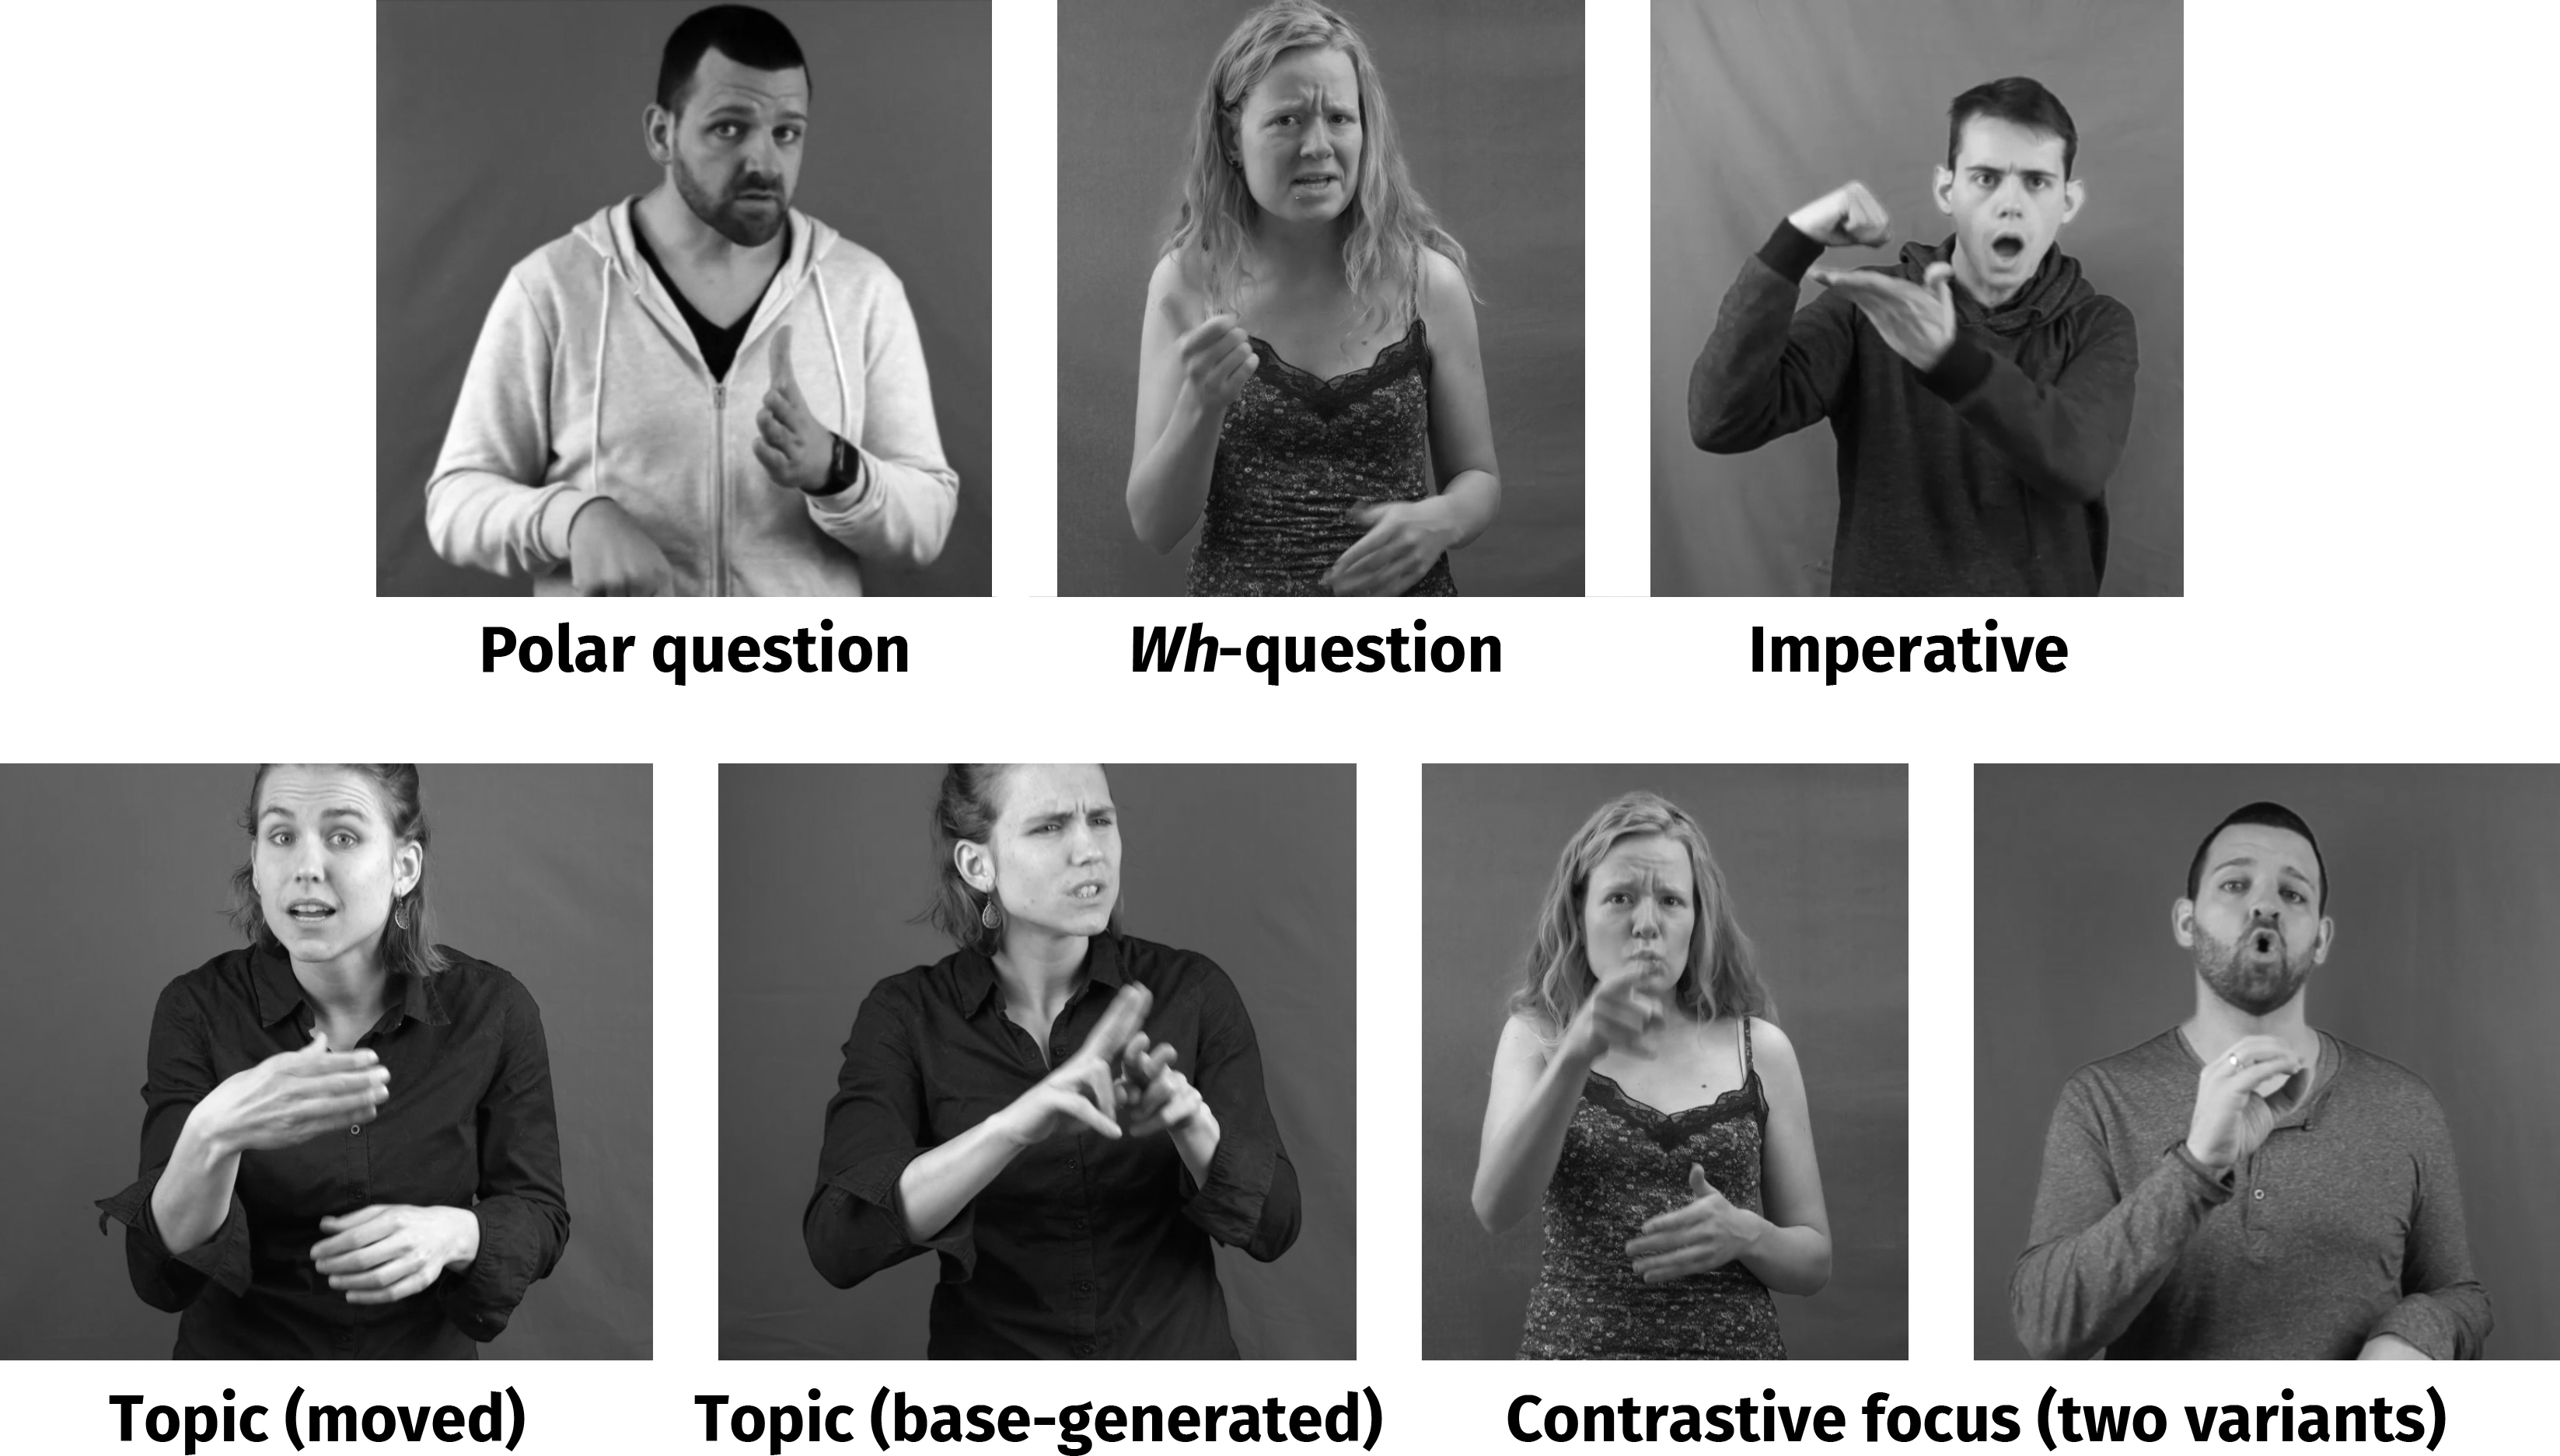
\includegraphics[width=1.0\textwidth]{uebersichtsw.jpg}
	\caption{All higher CP categories are expressed non-manually with the highest possible articulator, i.\,e., the eyebrows, sometimes together with other non-manuals. The upper row shows speech-act markings, the bottom row topic and focus marking (the expression of contrastive focus is subject to dialectal variation).}
	\label{highercpcategories}
\end{figure}

Indeed all categories above tense were found to be expressed non-manually only or by a combination of a manual sign plus a non-manual marker. All higher CP categories are expressed non-manually only in DGS: sentence types are encoded by using the eyebrows in DGS. While the same is true for moved and base-generated topics, focus marking involves several articulators including the head and, crucially, the eyes/eyebrows. Although contrastive focus was found to be subject to dialectal variation, both variants make use of the eyebrows. I have summarized the main non-manual markers used to express the higher CP categories in Figure \ref{highercpcategories}.

Additionally, all remaining categories above tense included in Cinque's system were found to be expressed either non-manually only or by a combination of non-manuals and manual signs. Two problematic cases were what Cinque called `irrealis mood'\is{irrealis mood} and `alethic modality' as both are categories which he puts below tense, but find non-manual expression with the upper face. In the case of irrealis mood (Section \ref{perhapsmoodirrealis}) I have argued, following \citet{nordstrom2010modality} and \citet{zyman2012two}, that irrealis mood and epistemic modality have the same distribution and both are structurally higher than tense. In the case of alethic modality\is{alethic modality} (Section \ref{alethicmodal}), I have argued, following \citet{palmer1986mood}, \citet{nuyts2000epistemic}, and \citet{von2006modality}, that it probably does not constitute a category on its own, but coincides with epistemic modality -- or, alternatively, that it is located above tense. This is in line with the finding that, similar to what has been described for spoken languages, there seems to be no difference in the expression of alethic and epistemic modality in DGS.

\begin{figure}[bt]
\centering
	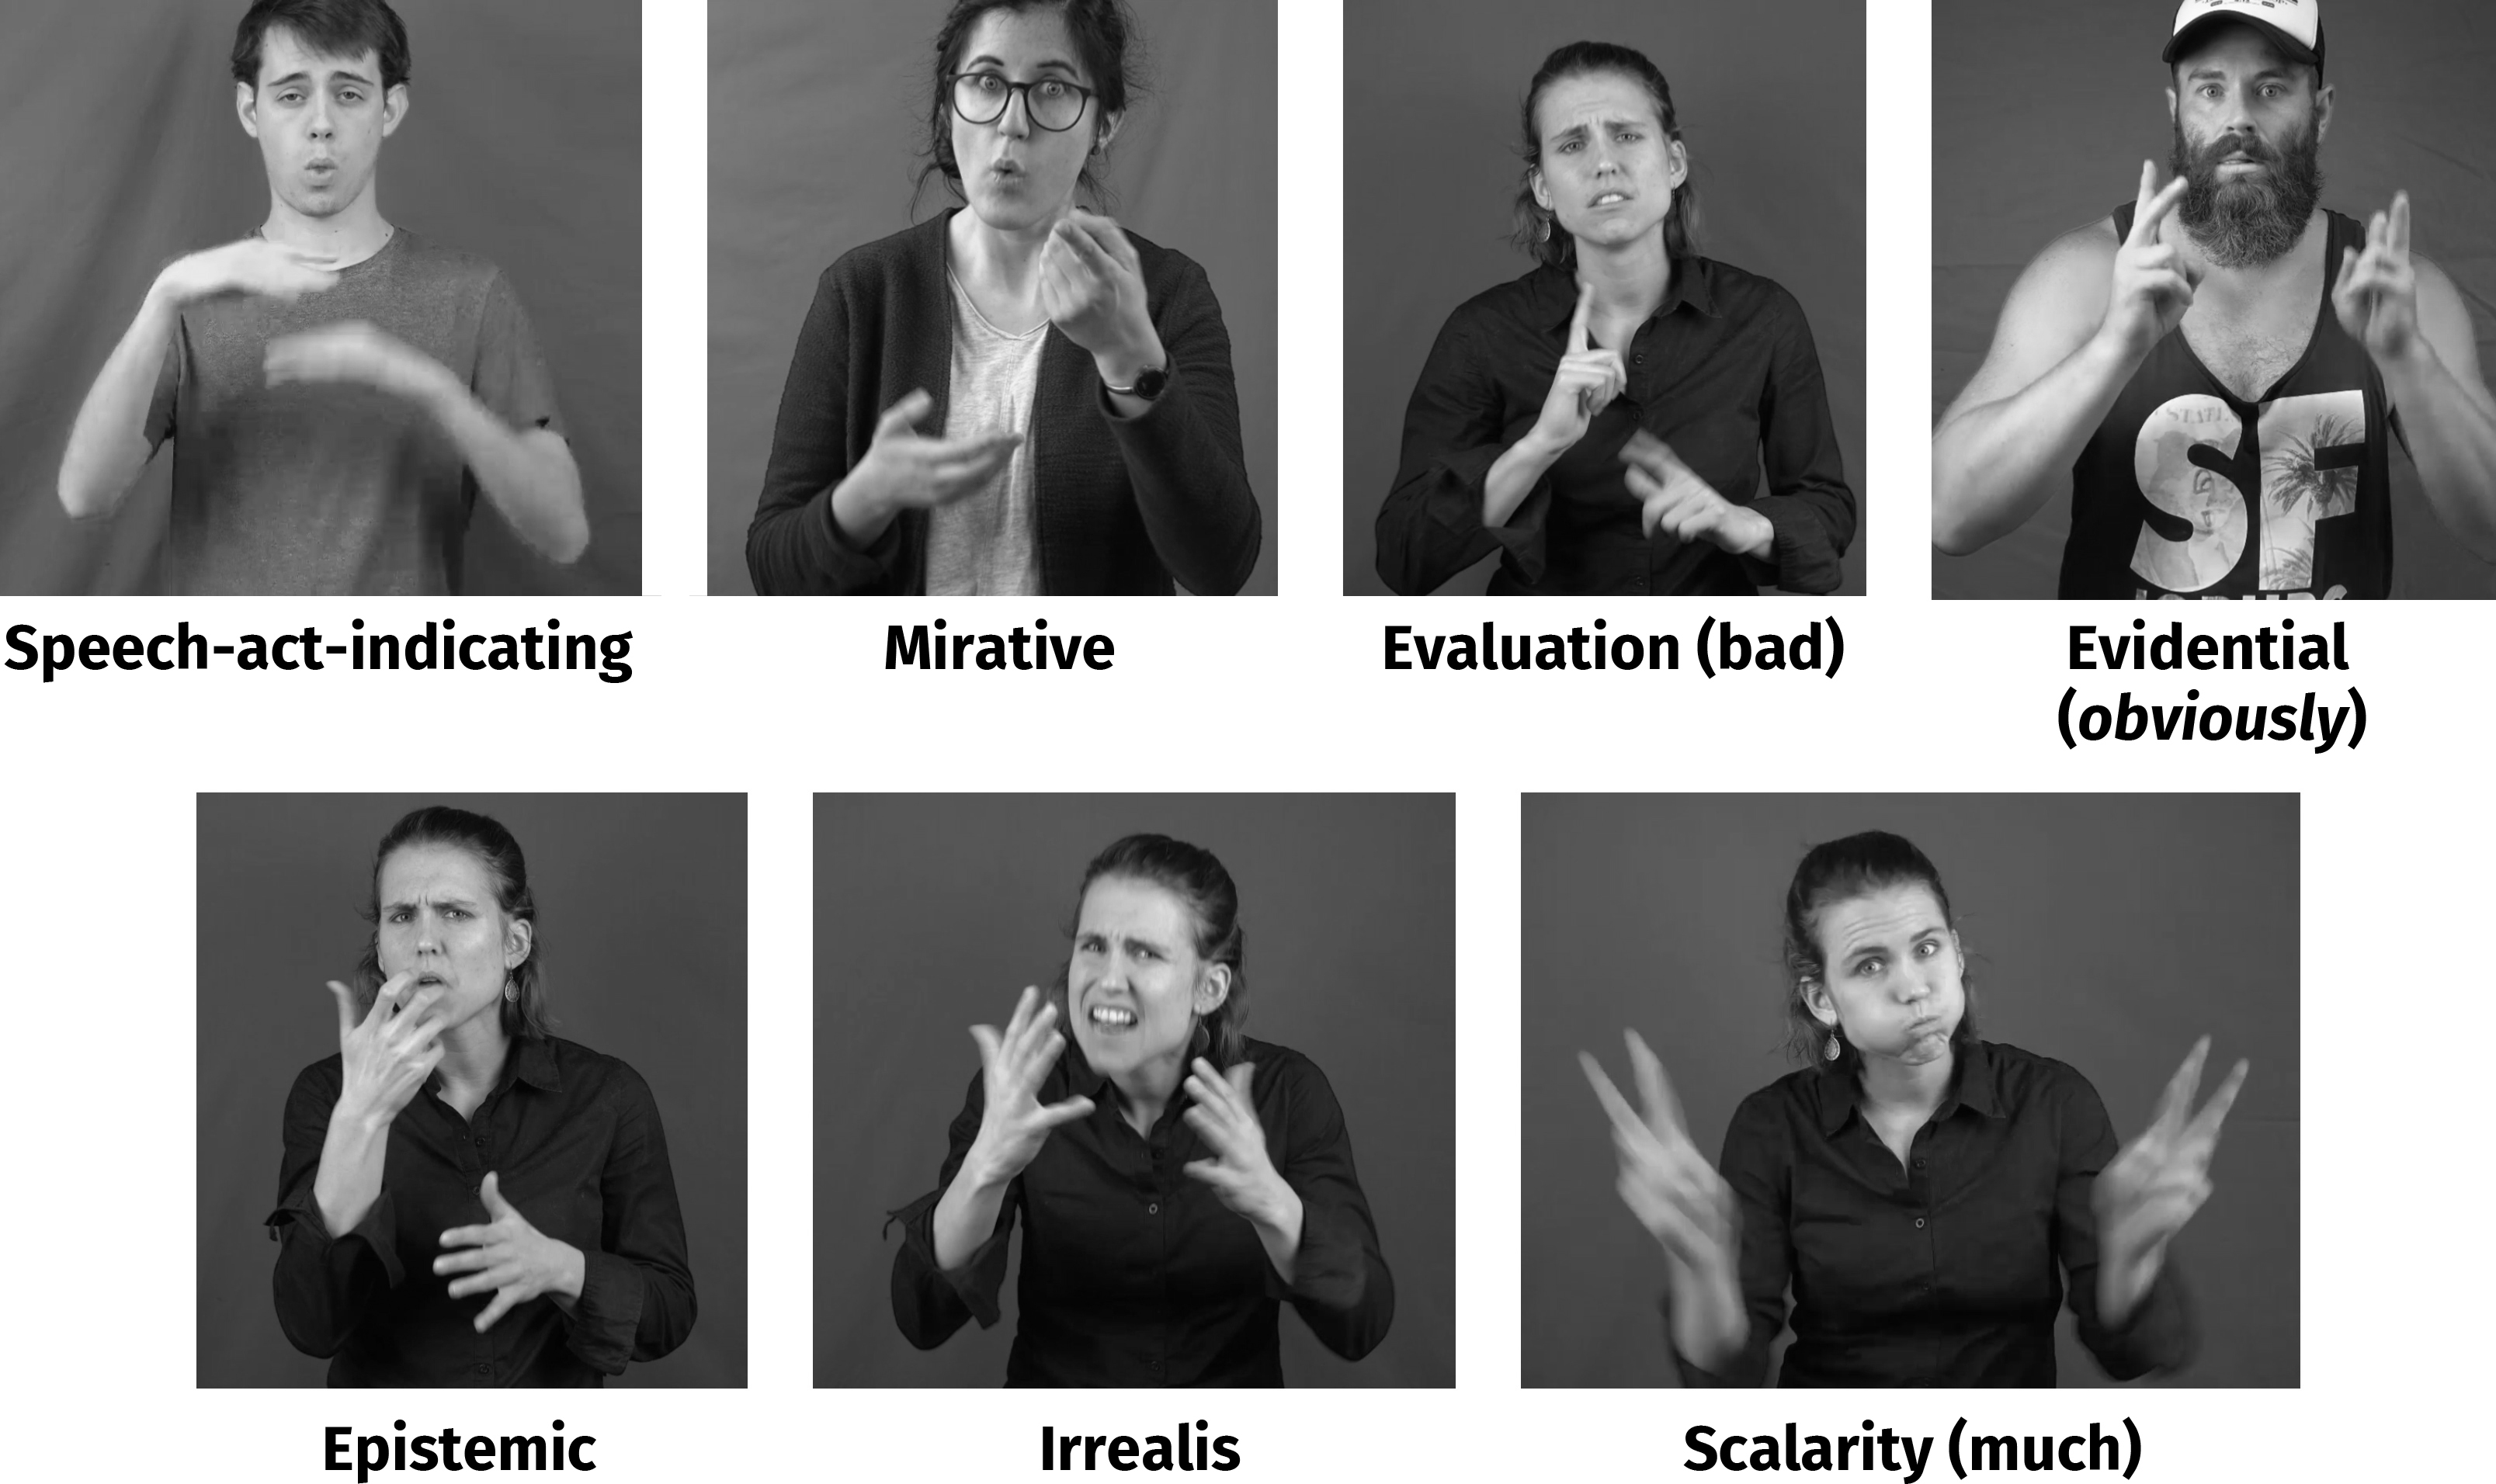
\includegraphics[width=1.0\textwidth]{uebersicht2sw.jpg}
	\caption{All Cinquean categories above tense find non-manual expression with the eyebrows and the eyes, sometimes together with other non-manuals.}
	\label{lowercpcategories}
\end{figure}

The higher Cinquean categories are expressed with the eyebrows or the eyes. Descending the hierarchy, one finds that scalarity (Section \ref{scalarity}) is produced by inflating or sucking in the cheeks. While DGS has no grammaticalized tense system, other sign languages which do have such a system use the shoulders to express tense (Section \ref{tense}). Both observations are in line with the idea of the bodily-mapping hypothesis. The non-manual markers used to express the higher categories in Cinque's system are depicted in Figure \ref{lowercpcategories}.

Taken together, all categories above tense are expressed non-manually. No category was found to take higher scope than another category, in which the former is expressed with a lower articulator than the latter. To the contrary, while most CP categories are expressed using the eyebrows, the lowest CP category, scalarity, is expressed by using a lower articulator, namely the cheeks. While the next lower category, tense, is not grammaticalized in DGS, temporal adverbs as well as all other IP- and VoiceP-internal categories are expressed with the lowest possible articulator, namely the hands. Thus, scope-taking in the clausal spine starts out with the eyebrows, descending the spine, scope-taking moves along the body on a vertical axis, through the cheeks (and the shoulders in some sign languages), then reaching the hands and finally switching to a strategy that incorporates categories into the movement path of manual signs. That neighboring categories are expressed by similar strategies is furthermore in line with the principle of analogical designation\is{analogical designation} stating that syntactic proximity is mirrored by phonological similarity. 

\is{bodily-mapping hypothesis|)}


\section{Concatenation strategies in DGS}\label{concatenatiostrategies}
While I claim that the bodily-mapping hypothesis may turn out to hold true in all sign languages, the question at which point in the clausal spine a language employs a left-to-right-concatenation or a right-to-left-concatenation strategy is thought to be subject to cross-linguistic variation -- just as in spoken languages. For (Southern) DGS it turned out that all categories below tense, but above the VoiceP level, find manual expression (without any layering). However, there were three exceptions to this generalization. In Section \ref{justjust} I described that the sign \textsc{just}, an instantiation of retrospective aspect\is{retrospective aspect}, is accompanied by a non-manual marker produced with the tongue. This deviation was explained by the assumption that this sign is always accompanied by the evaluation of a time interval as being little. Evidence for this claim comes from the fact that the intensity of the non-manuals can vary -- as a function how little the time interval is evaluated to be. In Section \ref{habitualaspect} I discussed that habitual aspect can be expressed through a manipulation of the movement path of the verb sign and in Section \ref{durativeaspect} I have shown that the same is true for durative aspect. In the case of habitual aspect expressed via \is{lower layering}lower layering I have shown that it should be taken as an instance of a lower scoping category as it cannot take scope above root modality (see Section \ref{habitualtwo})\is{habitual aspect}. A similar claim was made for durative aspect.

Taken together, I have argued that all IP-internal categories are expressed manually. Scope-taking generally proceeds from left to right as the natural landing site of the adverbs is to the left of the VP. This claim was supported by the fact that when two manual adverbs combine, the one with higher scope always precedes the one with lower scope. In contrast to what was claimed in \citet{bross2017scope}, the turning point from left-to-right to right-to-left concatenation was not found at root modality, but only with the lowest IP-internal category of manner adverbs (e.\,g., \textit{well}): the natural landing site of these adverbs is a post-verbal position. While modals show much more positional freedom (on the surface), the position of adverbs was found to be more restricted. Nevertheless, the combination of several modal verbs resulted in the predicted order (volitional modals, for example, have to precede root modals). 

\section{The at-issue/not-at-issue divide}\is{at-issue meaning|(}
In Section \ref{atnotissue} I have argued, following an idea by \citet{bross2017scope}, that the split between categories finding non-manual and categories finding manual expression is not only a split between the categories above and those below tense, but also a semantic split as the categories above tense contribute not-at-issue meaning while the categories below tense have a truth-conditional meaning contribution. While more empirical work has to be done in this domain, the presented results indicate that non-manual marking indeed generally contributes not-at-issue information. 

While this is clearly true for the higher CP categories which find non-manual expression only (e.\,g., speech-act markings), the picture with regard to the categories which can either be expressed non-manually only or by a combination of non-manual and manual expression (e.\,g., mirative marking) is more complex. In contrast to spoken English (or German), the manually signed adverbs were rated as contributing at-issue information by the signers I consulted. On the whole, the hypothesis that non-manuals express not-at-issue and manuals express at-issue meaning seems to be true. %The question whether higher (speaker-oriented) adverbs 



\is{at-issue meaning|)}


\section{The VoiceP-internal modulation hypothesis}
\is{VoiceP-internal modulation hypothesis|(}\is{lower layering|(}
In the previous chapter I have argued that all Cinquean categories below VoiceP find expression by lower layering, i.\,e., by manipulating the movement path of the verb sign. Problematic cases were what is called `habitual aspect' and `durative aspect' in the literature as both should belong to higher, IP-internal categories, but find expression by \is{lower layering}lower layering. In both cases, I have argued that these categories are indeed located below VoiceP (see also Section \ref{concatenatiostrategies} in this chapter). 


Taken together, I have found no counter-evidence for the idea that VoiceP-internal categories are expressed by single (manual) signs or even by higher articulators such as the eyebrows. Instead, all categories were found to be either expressed by lower layering\is{lower layering} (continuative II\is{continuative aspect II}, \is{celerative aspect II}celerative II, completive II, frequentative II) or have no grammaticalized expression in DGS at all (inceptive II\is{inceptive aspect II}, \is{repetitive aspect II}repetitive II). 


That the inner aspects are expressed by modulating the movement path of the verb sign is, in a sense, a case of iconicity and fits in well will the idea that there is some direct mapping of event structure and the morphological shape of a (manual) sign in sign languages in general, a proposal which has been called the \is{event visibility hypothesis}event visibility hypothesis (e.\,g., \citealt{wilbur2004event, wilbur2008complex, grose2007events}).



\is{VoiceP-internal modulation hypothesis|)}
\is{lower layering|)}


\section{Final remarks}
%It has been fun, but now I'm done!
%Ich hoffe, ein neues, fruchtbares Forschungsfeld eröffnet zu haben, das auch noch easy zu testen ist :)
I hope that this book has shown that the Cartography of sign languages is a fruitful and easy-to-conduct research approach. While many of the results presented in the previous chapters certainly need further investigation, I am confident that the general patterns will reproduce -- also in other sign languages. 



